%%%%%%%%%%%%%%%%%%%%%%%%%%%%%%%%%%%%%%%%%%%%%%%%%%%%%%%%%%%%%%%%%%%%%%%%%%%%%%%%
%%                          uAlberta Thesis Template                          %%
%%                                     by                                     %%
%%                               Daniel Aldrich                               %%
%%                               Version: 1.5.0                               %%
%%%%%%%%%%%%%%%%%%%%%%%%%%%%%%%%%%%%%%%%%%%%%%%%%%%%%%%%%%%%%%%%%%%%%%%%%%%%%%%%
%                                                                              %
%       Copyright (c) 2022 Daniel Aldrich                                      %
%                                                                              %
%       Permission is hereby granted, free of charge, to any person            %
%       obtaining a copy of this software and associated documentation         %
%       files (the "Software"), to deal in the Software without                %
%       restriction, including without limitation the rights to use,           %
%       copy, modify, merge, publish, distribute, sublicense, and/or           %
%       sell copies of the Software, and to permit persons to whom the         %
%       Software is furnished to do so, subject to the following               %
%       conditions:                                                            %
%                                                                              %
%       The above copyright notice and this permission notice shall be         %
%       included in all copies or substantial portions of the Software.        %
%                                                                              %
%       THE SOFTWARE IS PROVIDED "AS IS", WITHOUT WARRANTY OF ANY KIND,        %
%       EXPRESS OR IMPLIED, INCLUDING BUT NOT LIMITED TO THE WARRANTIES        %
%       OF MERCHANTABILITY, FITNESS FOR A PARTICULAR PURPOSE AND               %
%       NONINFRINGEMENT. IN NO EVENT SHALL THE AUTHORS OR COPYRIGHT            %
%       HOLDERS BE LIABLE FOR ANY CLAIM, DAMAGES OR OTHER LIABILITY,           %
%       WHETHER IN AN ACTION OF CONTRACT, TORT OR OTHERWISE, ARISING           %
%       FROM, OUT OF OR IN CONNECTION WITH THE SOFTWARE OR THE USE OR          %
%       OTHER DEALINGS IN THE SOFTWARE.                                        %
%                                                                              %
%%%%%%%%%%%%%%%%%%%%%%%%%%%%%%%%%%%%%%%%%%%%%%%%%%%%%%%%%%%%%%%%%%%%%%%%%%%%%%%%
%                                                                              %
%                                   NOTICE                                     %
% This template and class assume a basic understanding of how LaTeX works.     %
%                                                                              %
%%%%%%%%%%%%%%%%%%%%%%%%%%%%%%%%%%%%%%%%%%%%%%%%%%%%%%%%%%%%%%%%%%%%%%%%%%%%%%%%
%                                                                              %
% To use this template start by entering in your information in the fields     %
%     below, and in the file `ualberta.xmpdata'. Next remember to delete the   %
%     auto generated text `\lipsum[##]'.                                       %
%                                                                              %
% Most LaTeX packages required have already been included in this document     %
%     document class.                                                          %
%                                                                              %
% For referencing, use the command \Cref{<label>} for smart referencing that   %
%     includes the type of reference, i.e., for a figure it will produce the   %
%     the text `Figure #.#'.                                                   %
%                                                                              %
% Compact citations can be made by using a single \cite command, e.g.:         %
%     `\cite{ref1, ref2, ref3,...}.                                            %
%                                                                              %
%%%%%%%%%%%%%%%%%%%%%%%%%%%%%%%%%%%%%%%%%%%%%%%%%%%%%%%%%%%%%%%%%%%%%%%%%%%%%%%%

% INCLUDES PACKAGES:
% array, nomencl, etoolbox, lipsum, xmpincl, xcolor, graphicx, tabularx, 
% makecell, subcaption, rotating, booktabs, multicol, multirow, amsmath, 
% amsfonts, amssymb, pdflscape, textcomp, longtable, listings, pdfpages
% pgfplots, xparse, ifthen, hyphenat, hyperref, cleveref, inputenc
% 
% For a full description of each of the included packages please read the 
%  packages file.

%LIST OF DEFINED SYMBOLS
  % For the full list of symbols included please see `includeSymbols.tex'
	%\regTM                %Registered Trademark\regTM
	%\nonTM                %Unregistered Trademark
	%\cRight{}             %Copyright
	%\cLeft{}              %Copyleft
	%\degrees{}            %Degrees
	%\hyph{}               %Hyphen
	%\latin{<text here>}   %Latin
	%\etal{}               %et al.
	%\etc{}                %etc
	%\eg{}                 %e.g.
	%\ie{}                 %i.e.
	%\Kevlar{}             %Kevlar
	%\Matlab{}             %Matlab

%LIST OF AVAILABLE THEOREM ENVIRONMENTS
  % For the full list of theorems included please see `includeTheroems.tex'
	% theorem, algorithm, axium, case, claim, conclusion, condition, 
	% conjecture, corollary, criterion, definition, example, exercise, 
	% lemma, notation, problem, proposition, remark, solution, summary
	%
	% To use:
	% \begin{<theorem name>}
	%     <YOUR TEXT HERE>
	% \end{<theorem name>}
        
%LIST OF USEFUL COMMANDS:
	%\comment{}            %Nothing inside the braces will be printed
	%\nonumeq{}            %Un-numbered, centered equation.
	%\numeq{}{label}       %Numbered, centered equation.
	%\brackS{}             %Surrounds the input with []
	%\brackR{}             %Surrounds the input with ()
	%\brackC{}             %Surrounds the input with {}

%FOR TABLES OF A SPECIFIC WIDTH USE:
	% It is recommended to use the tabularx package
	% Further, to provide a more professional look to your tables do not use vertical
	%   lines. Instead use \toprule, \midrule, and \bottomrule to make the horizontal
	%   lines. 
	%
	% See the Chapters\ExampleChapter.tex for examples on how to make your tables and
	%   figures.

% INCLUDING CODE
	% To include code or code snippets in your thesis, the package listings is used.
	% A number of predefined code highlighting schemes are included in the file
	%   `listingCodeFormatting.tex' including:
	%   Matlab, C/C++, VB/VBA, and XML 
	%
	% Examples of how to include code are shown in Appendix C

\immediate\write18{makeindex \jobname.nlo -s nomencl.ist -o \jobname.nls}
% Write command to allow the nomenclature to be generated properly.


\documentclass[pdfa,chapterbib]{ualberta}
% OPTIONS FOR ualberta.cls:
% chapterbib - \printreferences now prints references at the end of a chapter
% 
% pdfa - to convert the pdfa to PDF/A format
% 
% oneside - Standard for submitting to FGSR.
% 
% twoside - If you want to print your thesis double sided like a novel.

%%%%%%%%%%%%%%%%%%%%%%%%%%%%%%%%%%%%%%%%%%%%%%%%%%%%%%%%%%%%%%%%%%%%%%%%%%%%%%%%
%                  TITLE PAGE AND FRONTMATTER INFORMATION                      %
%%%%%%%%%%%%%%%%%%%%%%%%%%%%%%%%%%%%%%%%%%%%%%%%%%%%%%%%%%%%%%%%%%%%%%%%%%%%%%%%
% TITLE PAGE INFO
 \title{Thesis Title}              % Title of your Thesis
 \author{First Middle Last}        % Your Full Name
 \degree{\MSc}                     % \MSc, \PhD, \MA, \MEd, \MBA, \MAc, \MFM, \MN, \LLM, or \MMus
 \specialization{}                 % Leave blank if none
 \department{Example Department}   % Fill in the Department unless you are non-Departmental
 \faculty{}                        % Leave blank unless non-Departmental
 \convocationdate{2022}            % Convocation Year

% Don't forget to edit ualberta.xmpdata with the same metadata for the PDF/A

% ABSTRACT
  \abstracttext{%
    A thesis must have an abstract. 
    The abstract comes after the title page and is marked page ``ii''.

    The abstract is a concise and accurate summary of the thesis. 
    It states the problem that was researched, the methods of investigation, and the general conclusions. 
    An abstract must not contain non-text content, such as tables, graphs, complex equations, or illustrations.
    Even for theses containing journal articles, there is one single abstract for the entire work, included within the preliminary pages (front pages) of the thesis.

    For any thesis that is permitted to be written in a language other than English, two abstracts must be included; the first in English and the second in the language of the thesis.

    The font used for the abstract must be at least a 10 point font, with the text double-spaced, to ensure readability. 
    A strict maximum word count of 700 words applies, regardless of whether the abstract is for a master's or a doctoral degree (many abstracts are 300--500 words).

    For refernece this section is exactly one-hundred and seventy-six words.
	}

% PREFACE
  % Requirements
  \preface{
    \textbf{If you need assistance on writing the preface, ask your supervisor.
    Your supervisor must review and verify the preface before it becomes part of the final version of the thesis.}

    A preface is a mandatory component of a thesis, regardless of thesis format, \underline{when} a thesis contains journal articles authored or co-authored by the student (including an accepted paper that is forthcoming at the time of thesis submission). 
    A preface is \underline{also} a mandatory component when the research conducted for the thesis required ethics approval. 
    A preface remains optional if there is no inclusion of journal articles and/or no need for ethics approval.
    
    When required because a thesis contains journal articles, the preface serves as a place for the student to include a statement indicating his or her contribution to the journal articles, such as the identification and design of the research program, the performance of the various parts of the research (including the collection of data, construction of any necessary apparatus, and the performance of experiments), and the analysis of the research data. 
    If any of the work presented in the thesis has led to any publications (accepted or published), these publications must be listed clearly in the preface with their bibliographical details and an indication as to where in the thesis this work is located (e.g. state in which chapter or chapters). 
    For jointly authored publications, indication must also be given as to the relative contributions of the collaborators and co-authors, and a statement as to the proportion of research and writing conducted by the student. 
    Note that permission may be needed if the co-authors hold the copyright in these publications. 
    If ethics approval was required for the research, a statement to this effect must be included in the preface with the details of the approval that was granted. 
    
    Note that the inclusion of a preface does not excuse a student from failing to acknowledge the contributions of others in the body of the thesis, as per the University's Research and Scholarship Integrity Policy and the Code of Student Behaviour. One would still expect to see footnotes, endnotes or in-text references within the thesis acknowledging the works. Acknowledgments, such as thanks to the supervisor and supervisory committee members, to colleagues, lab mates and friends, and to family, do not appear in the preface. 
    
    \textbf{Examples of several prefaces are given in Appendix B and are also available from the FGSR website.}
   }
   
  % Optional
    %\preface{%
      %This thesis is an original work by `Your name here'. No part of this thesis has been previously published.
    %}
    
  % Mandatory due to research ethics approval
    %\preface{
      %This thesis is an original work by `Yourname here'. 
      %The research project, of which this thesis is a part, received research ethics approval from the University of Alberta Research Ethics Board, Project Name “TITLE”, No. 12345, DATE.
    %}
    
  % Mandatory due to collaborative work
    %\preface{%
      %Some of the research conducted for this thesis forms part of an international research collaboration, led by Professor R.C. Smith at the University of Hogwarts, with Professor D.R. Brown being the lead collaborator at the University of Alberta. 
      %The technical apparatus referred to in chapter 3 was designed by myself, with the assistance of M.C. White and Professor D.R. Brown. 
      %The data analysis in chapter 4 and concluding analysis in chapter 5 are my original work, as well as the literature review in chapter 2.
      %
      %Chapter 3 of this thesis has been published as J.D. Doe, M.C. Smith, and R.C. Smith, “Theoretical Responses to Rays in the Gamma System,” Journal of Scientific Affairs, vol. 165, issue 3, 459-475. 
      %I was responsible for the data collection and analysis as well as the manuscript composition. 
      %M.C. Smith assisted with the data collection and contributed to manuscript edits. R.C. Smith was the supervisory author and was involved with concept formation and manuscript composition. 
    %}
  
% DEDICATION
  % Dedications, quotations, poems etc are optional. 
  % Ask your supervisor for advice or views on whether to include such matters in an academic work, with the next component serving as the place to thank people.
	\thesisquote{``\lipsum*[14]{}''\\-Author of the Quote}
	\dedication{To...}

% ACKNOWLEDGMENTS
	\acknowledgementtext{%
		An Acknowledgements page (no more than 2 pages in length) is a recommended, but not mandatory, component of a thesis.
		
		The Acknowledgements page serves as a place within a thesis where students may wish to acknowledge the provision of funding from third parties, such as an external scholarship bodies, research granting agencies, and foreign governments. 
		It is also appropriate to recognize the assistance provided by the supervisor and members of the supervisory committee.
		
    \latin{e.g. } I would like to thank Daniel R. Aldrich for his continuing contributions to the University of Alberta, and for his work within the graduate student community. More specifically, I would like to acknowledge the work that he put into creating the \LaTeX{} template that this thesis was created in, and the ongoing support that he provides to the students at the University of Alberta.
		\lipsum[2-5]
	}


%%%%%%%%%%%%%%%%%%%%%%%%%%%%%%%%%%%%%%%%%%%%%%%%%%%%%%%%%%%%%%%%%%%%%%%%%%%%%%%%
%                  NOMENCLATURE, GLOSSARY, ACRONYMS, ETC                       %
%%%%%%%%%%%%%%%%%%%%%%%%%%%%%%%%%%%%%%%%%%%%%%%%%%%%%%%%%%%%%%%%%%%%%%%%%%%%%%%%

% NOMENCLATURE
 % Note: Nomenclature is automatically sorted alphabetically
 % [A] : Constants
 % [B] : Latin
 % [C] : Greek
 % Use \nomunit{$Value\, Units$} to add the value and units for a defined constant

 \nomenclature[A]{$c$}{Speed of light in a vacuum inertial system.\nomunit{$299,792,458\, m/s$}}
 \nomenclature[A]{$h$}{Planck constant.\nomunit{$6.62607015E-34\, Js$}}
 \nomenclature[B]{$E$}{Elastic Constant (Young's Modulus)}
 \nomenclature[B]{$T$}{Torque}
 \nomenclature[B]{$a$}{Acceleration}
 \nomenclature[B]{$v$}{Velocity}
 \nomenclature[B]{$m$}{Mass}
 \nomenclature[C]{$\varepsilon$}{Strain}
 \nomenclature[C]{$\alpha$}{Primary Angle}

% ACRONYMS (Do NOT include periods at the end)
 % Note: Acronyms are automatically sorted alphabetically
 \addacronym{ROFL}{Rolling on floor laughing}
 \addacronym{STFU}{Shut the *swear word!* up}
 \addacronym{ICYMI}{In case you missed it}
 \addacronym{TL;DR}{Too long, didn't read}
 \addacronym{LMK}{Let me know}
 \addacronym{NVM}{Nevermind}
 \addacronym{TGIF}{Thank goodness it's Friday}
 \addacronym{TBH}{To be honest}
 \addacronym{TBF}{To be frank}
 \addacronym{RN}{Right now}
 \addacronym{QOTD}{Quote of the day}
 \addacronym{OOTD}{Outfit of the day}
 \addacronym{BRB}{Be right back}
 \addacronym{BTW}{By the way}
 \addacronym{LOL}{Laugh out loud}
 \addacronym{TTYL}{Talk to you later}
 \addacronym{HMU}{Hit me up}
 \addacronym{FWIW}{For what it's worth}
 \addacronym{IMO}{In my opinion}
 \addacronym{IMHO}{In my humble opinion}
 \addacronym{IDK}{I don't know}
 \addacronym{TBA}{To be announced}
 \addacronym{TBD}{To be decided}

% GLOSSARY (Do NOT include periods at the end)
 % Note: Glossary is automatically sorted alphabetically
 \addterm{Strength (STR)}{The character's physical strength. This effects the potency of melee attacks}
 \addterm{Dexterity (DEX)}{Agility and accuracy. This affects ranged attacks and dodging}
 \addterm{Constitution (CON)}{Physical resilience. This affects hit points and some physical resistances}
 \addterm{Intelligence (INT)}{The ability to process problems and wield certain magic. INT affects the number of skill points received}
 \addterm{Wisdom (WIS) }{Common sense and spirituality}
 \addterm{Charisma (CHR)}{Social skills and sometimes physical appearance}
 \addterm{Good}{Having a respect for life, altruism, and selflessness}
 \addterm{Evil}{Wicked and often selfish or oppressive}
 \addterm{Lawful}{Abides by a core morality or honor system. Can also be judgmental and close-minded}
 \addterm{Chaotic}{Free-spirited and sometimes unpredictable. Can also be reckless or reactionary}
 \addterm{Neutral}{A balance between Lawful \& Chaotic or Good \& Evil}

% BIBLIOGRAPHY LOCATION
 % NOTE: if you add bibliography entries after a compilation, you might notice 
 %   references marked `[0]' to fix this just delete the auxiliary files. (*.aux, *.bbl, ... etc)
  % .  - This folder
  % .. - Up one Folder
 \addbibresource{./References/References.bib}


%%%%%%%%%%%%%%%%%%%%%%%%%%%%%%%%%%%%%%%%%%%%%%%%%%%%%%%%%%%%%%%%%%%%%%%%%%%%%%%%
%                              BEGIN DOCUMENT                                  %
%%%%%%%%%%%%%%%%%%%%%%%%%%%%%%%%%%%%%%%%%%%%%%%%%%%%%%%%%%%%%%%%%%%%%%%%%%%%%%%%
\begin{document}

 \maketitle                    % Creates the title page
 \makeabstract                 % Creates the abstract
 \makepreface                  % Uncomment line to add Preface Page
 %\makequote                   % Uncomment line to add Quote Page
 %\makededication              % Uncomment line to add Dedication Page
 \acknowledgements             % Uncomment line to add Acknowledgements

% SET ToC...etc SPACING
 %\singlespacing               % 1.00x Spacing
 \onehalfspacing              % 1.50x Spacing
 %\doublespacing               % 1.75x Spacing
 %\truedoublespacing            % 2.00x Spacing
 %\triplespacing               % 3.00x Spacing
 %\baselineskip #.##em         % #.##x Spacing

 \tableofcontents              % Create the Table of Contents
 \listoftables                 % Uncomment line if you have tables
 \listoffigures                % Uncomment line if you have figures
 \listofplates                 % Uncomment line if you have plates (photographs)
 \listofsymbols                % Uncomment if you have a List of Symbols (Nomenclature)
 \abbreviations                % Uncomment if you have a Abbreviations (List of Acronyms)
 \glsaddall                    % Required for List of Acronyms and Glossary (DO NOT COMMENT)
 \generateglossary             % Uncomment if you have Glossary of Terms

%%%%%%%%%%%%%%%%%%%%%%%%%%%%%%%%%%%%%%%%%%%%%%%%%%%%%%%%%%%%%%%%%%%%%%%%%%%%%%%%
%                           ADD YOUR CONTENT HERE                              %
%%%%%%%%%%%%%%%%%%%%%%%%%%%%%%%%%%%%%%%%%%%%%%%%%%%%%%%%%%%%%%%%%%%%%%%%%%%%%%%%
 \bodyoftext                   % Switches the style of the document to that required for the body

% SET DOCUMENT SPACING
 %\singlespacing               % 1.00x Spacing **Allowed for FOOTNOTES and LONG QUOTES**
 %\onehalfspacing              % 1.50x Spacing **Minimum Spacing for the THESIS BODY**
 %\doublespacing               % 1.75x Spacing
 \truedoublespacing            % 2.00x Spacing **Required for the ABSTRACT**
 %\triplespacing               % 3.00x Spacing
 %\baselineskip #.##em         % #.##x Spacing

% NOTE: CHAPTER 2 PROVIDES SOME EXAMPLES OF TABLES, FIGURES, AND EQUATIONS

% Though the following chapters are written in this tex file, it is highly recommened to 
%   separate chapters into their own files. 
\chapter{Introduction}\label{ch:Introduction}
  The first page of the introduction is marked as page ``1'' and then the pages that follow are numbered sequentially.

  The minimum academic requirements for the text of a thesis are an introduction, followed by the presentation of the research in a manner suitable for the field, and a conclusion.

  The introduction must outline the thesis, problem, hypothesis, questions or goals of the research.
  It must provide a clear statement of the research question(s).
  The conclusion must highlight the student’s contribution to knowledge, providing conclusions with respect to the problem, hypothesis or goals of the research.
  In all theses, regardless of format, the body or chapters of the thesis contain methodology, research results, and scholarly discussion in accordance with the norms of the academic discipline.

  The University of Alberta encourages students to publish.
  Thus, one or more chapters of a thesis may contain published material if permitted by the regulations of your department (or Faculty if non-departmentalized) governing your specific degree program.
  It is a matter for individual graduate programs to develop specific guidance for students and supervisors, as well as supervisory committee members, with such specific guidance likely to reflect the needs of the particular field or academic discipline.

  For example, individual graduate programs that continue to prefer the traditional monograph-style thesis may have department-specific rules on such matters as maximum length (taking into account the burden on an external examiner to read a thesis that is over 100,000 words).
  Individual graduate programs that opt for a multiple-manuscript or journal-article format, or choose to accept both traditional and paper-based formats, or a combination of both, must have department-specific guidelines in place to address potential student and supervisor queries.
  For example, the department-specific guidance needs to address what counts as a publication (\latin{e.g. } self-publication, any journal, or only journals listed in a particular source); whether a paper-based thesis can include both published and accepted papers; whether the student must be the first author for a multiple-authored publication to be acceptable for inclusion within the thesis; and whether some form of connecting text is needed to link the papers beyond the introduction (and if so, what form or forms of connectors are acceptable).

  \section{Motivation}\label{sec:Motivation}
    \lipsum[1-3]
  \section{Thesis Objectives}\label{sec:thesisObjective}
    \lipsum[14-16]
  \section{Thesis Outline}\label{sec:thesisOutline}
    \lipsum[17]

% To insert chapters from a seperate tex file use the following commands
% \insertchapter automatically looks in the Chapters folder and also
%   appends the file extension (i.e. do NOT include the '.tex')
\insertchapter{ExampleChapter}

% \input is the standard way of including a seperate tex file
% \chapter{Example Chapter}\label{ch:Example}
  This chapter aims to provide examples how how to structure and create specific components in your thesis document. The very first one is showing a citation, like the one at the end of this sentence \cite{TEST}. The second shows how to create more than one citation and how they are grouped \cite{testone,cite2,cite3,cite4,cite5}.
This sentence shows how a gap in the citations is handled \cite{testone,cite2,cite3,cite5}. 
  \section{Tables}
  
  % L - Left Aligned (Equal Spacing)
  % C - Center Aligned (Equal Spacing)
  % R - Right Aligned (Equal Spacing)
  % l - Left Aligned (Fit to Contents)
  % c - Center Aligned (Fit to Contents)
  % r - Right Aligned (Fit to Contents)
  
  \begin{table}[!htb]
    \caption{This is a basic table}
    \centering
    \begin{tabularx}{0.75\textwidth}{LCR} 
      % Equally spaced cells that are left, center, and reight aligned. 
      % The entire table will be 75% the width of the text.
      \hline
      \textbf{Left Aligned Title} & \textbf{Centered Title} & \textbf{Right Aligned Title} \\\hline
      This is left aligned & This is centered & This is right aligned \\
      This is left aligned & This is centered & This is right aligned \\
      This is left aligned & This is centered & This is right aligned \\
      This is left aligned & This is centered & This is right aligned \\\hline
    \end{tabularx}
    \label{tab:basicTable}
  \end{table}
  
  \begin{table}[!htb]
    \caption{This is a complex table.}
    \centering
    \begin{tabularx}{\textwidth}{lCR}
      % Left most cell is fitted to the content.
      % The center and right columns are equally spaced cells that are center, and reight aligned. 
      % The entire table will be 75% the width of the text.
      \hline
      \multirow{2}{*}{\textbf{This is two row\quad}} & \multicolumn{2}{c}{\textbf{This is two columns}}\\\cline{2-3} % \cline draws a partial line across cells #-#
       & \textbf{Centered Title} & \textbf{Right Aligned Title} \\\hline
      \multirow{2}{*}{This is two row} & This is centered & This is right aligned \\
       & This is centered & This is right aligned \\\cline{1-1}
      \multirow{2}{*}{This is two row} & This is centered & This is right aligned \\
       & This is centered & This is right aligned \\\hline
    \end{tabularx}
    \label{tab:complexTable}
  \end{table}
  
  
  \section{Figures}
  This section will provide examples of how to create figures, and different types of multi/sub-figures. Additionally, if you have many figures in a section and they are bleeding too much into the following sections a \textbackslash{}clearpage command can be issued before the next section. However, note that this will force the next section to begin on a new page. Note that the first ``figure'' is actually a plate; a plate is the proper title associated with a photograph, using the environment `plate' instead of figure and command listofplates will generate everything for you.
  \begin{plate}[!htb]
    \centering
    \includegraphics[width=0.7\textwidth]{example-image}
    \caption{This is an example of a single image plate.}
    \label{fig:singleImage}
  \end{plate}
  
  \begin{figure}[!htb]
    \centering
    \begin{subfigure}{0.45\textwidth}
      \includegraphics[width=\textwidth]{example-image}
      \caption{} % Leave blank for just letter
      \label{fig:doubleImage:a}
    \end{subfigure}
    ~
    \begin{subfigure}{0.45\textwidth}
      \includegraphics[width=\textwidth]{example-image}
      \caption{} % Leave blank for just letter
      \label{fig:doubleImage:b}
    \end{subfigure}
    \caption{This is an example of a double image figure.}
    \label{fig:doubleImage}
  \end{figure}
  
  \begin{figure}[!htb]
    \centering
    \hspace*{\fill}% Adds space to left of top image (prevents two images from going to top)
    \begin{subfigure}{0.45\textwidth}
      \includegraphics[width=\textwidth]{example-image}
      \caption{} % Leave blank for just letter
      \label{fig:tripleImage:a}
    \end{subfigure}
    \hspace*{\fill} % Adds space to right of top image (prevents two images from going to top)
    \par\vspace{1em}% Adds space between upper and lower images
    \begin{subfigure}{0.45\textwidth}
      \includegraphics[width=\textwidth]{example-image}
      \caption{} % Leave blank for just letter
      \label{fig:tripleImage:b}
    \end{subfigure}
    ~ % Adds space between the two lower figures
    \begin{subfigure}{0.45\textwidth}
      \includegraphics[width=\textwidth]{example-image}
      \caption{} % Leave blank for just letter
      \label{fig:tripleImage:c}
    \end{subfigure}
    \caption{This is an example of a triple image figure.}
    \label{fig:tripleImage}
  \end{figure}
  
  \begin{figure}[!htb]
    \centering
    \hspace*{\fill}% Adds space to left of top image (prevents two images from going to top)
    \begin{subfigure}{0.90\textwidth+1em} % 0.9 = 0.45 + 0.45, and 1em is the width of ~
      \includegraphics[width=\textwidth]{example-image}
      \caption{} % Leave blank for just letter
      \label{fig:tripleImage:a}
    \end{subfigure}
    \hspace*{\fill} % Adds space to right of top image (prevents two images from going to top)
    \par\vspace{1em}% Adds space between upper and lower images
    \begin{subfigure}{0.45\textwidth}
      \includegraphics[width=\textwidth]{example-image}
      \caption{} % Leave blank for just letter
      \label{fig:tripleImage:b}
    \end{subfigure}
    ~ % Adds space between the two lower figures
    \begin{subfigure}{0.45\textwidth}
      \includegraphics[width=\textwidth]{example-image}
      \caption{} % Leave blank for just letter
      \label{fig:tripleImage:c}
    \end{subfigure}
    \caption{This is a second example of a triple image figure.}
    \label{fig:tripleImage}
  \end{figure}
  
  \begin{figure}[!htb]
    \centering
    \begin{subfigure}{0.45\textwidth}
      \includegraphics[width=\textwidth]{example-image}
      \caption{} % Leave blank for just letter
      \label{fig:quadImage:a}
    \end{subfigure}
    ~ % Adds space between the two top figures
    \begin{subfigure}{0.45\textwidth}
      \includegraphics[width=\textwidth]{example-image}
      \caption{} % Leave blank for just letter
      \label{fig:quadImage:b}
    \end{subfigure}
    \par\vspace{1em} % Adds space between upper and lower images
    \begin{subfigure}{0.45\textwidth}
      \includegraphics[width=\textwidth]{example-image}
      \caption{} % Leave blank for just letter
      \label{fig:quadImage:c}
    \end{subfigure}
    ~ % Adds space between the two lower figures
    \begin{subfigure}{0.45\textwidth}
      \includegraphics[width=\textwidth]{example-image}
      \caption{} % Leave blank for just letter
      \label{fig:quadImage:d}
    \end{subfigure}
    \caption{This is an example of a quad image figure.}
    \label{fig:quadImage}
  \end{figure}
  
  \clearpage % forces the remaining images (floats to be placed)
  \section{Equations}
  The following equation has no referencing number:
  \nonumeq{E = & m\ c^2}
  
  \Cref{eq:quickEq} has a reference to it though. Or for more control the source for \Cref{eq:quickEq} can be written out fully as it was for \Cref{eq:quickEq2}.
  
  \numeq{pi = & 3.1415...}{eq:quickEq} % shorthand for the following way of writing equations.
  \begin{align}\label{eq:quickEq2}
    e = & 2.7183...
  \end{align}
  
  If you have multiple equations that you want arranged very neatly, use the align environment and you can assign individual equations numbers as shown in \Cref{eq:multiref:a,eq:multiref:b,eq:multiref:c}.
  \begin{align}%Note: Alignment happens at the "=" character
    \label{eq:multiref:a} Equation1 = & 1 + 1\\
    \label{eq:multiref:b} Equation2 = & 2 + 2\\
    \label{eq:multiref:c} Equation3 = & 3 + 3
  \end{align}
  
  
  
  \printreferences % Add a Reference Section to the end of the Chapter.
                
\chapter{Background}\label{ch:Background}
  \section{General Information}\label{sec:generalInformation}
    \lipsum[23-25]
  \section{Specific Information}\label{sec:specificInformation}
    \lipsum[35-37]
  \section{Gap in Research}\label{sec:gapInResearch}
    \lipsum[42-43]
  \section{Conclusions}\label{sec:backgroundConclusions}
    \lipsum[12-13]

\chapter{Paper 1}\label{ch:Paper1}
  \section{Introduction}\label{sec:P1Introduction}
    \lipsum[34-36]
  \section{Methods and Procedure}\label{sec:P1methodsAndProcedure}
    \begin{case}
      \lipsum[10]
    \end{case}
    \begin{case}
      \lipsum[15]
    \end{case}
    \lipsum[46-48]
  \section{Results and Discussion}\label{sec:P1resultsAndDiscussion}
    \lipsum[55-57]
  \section{Conclusions}\label{sec:P1Conclusions}
    \lipsum[12-13]
                
\chapter{Paper 2}\label{ch:Paper2}
  \section{Introduction}\label{sec:P2Introduction}
    \lipsum[34-36]
  \section{Methods and Procedure}\label{sec:P2methodsAndProcedure}
    \lipsum[46-48]
  \section{Results and Discussion}\label{sec:P2resultsAndDiscussion}
    \lipsum[55-57]
  \section{Conclusions}\label{sec:P2Conclusions}
    \lipsum[12-13]
                
\chapter{Conclusions, Recommendations, \& Future Work}\label{ch:Conclusions}
  \section{Conclusions}\label{sec:Conclusions}
    \lipsum[34-36]
  \section{Future Work}\label{sec:futureWork}
    \lipsum[38]\cite{TEST}
	
  % \printreferences Prints a reference section at the end of the current chapter
  %
  % If the `chapterbib' option is not declaired, \printreferences does nothing
  %    This allows you to turn end of chapter references on and off easily.
  %
  % Note: End of chapter references share references with the Bibliography that
  %    is REQUIRED at the end of your thesis, so the numbering of the end of 
  %    chapter references may not start at 1 and may not increment by one.
  \printreferences 

%%%%%%%%%%%%%%%%%%%%%%%%%%%%%%%%%%%%%%%%%%%%%%%%%%%%%%%%%%%%%%%%%%%%%%%%%%%%%%%%
%                                 BIBLIOGRAPHY                                 %
%%%%%%%%%%%%%%%%%%%%%%%%%%%%%%%%%%%%%%%%%%%%%%%%%%%%%%%%%%%%%%%%%%%%%%%%%%%%%%%%

% These two lines make sure that the bibliography starts on a new page.
\bigskip 
\clearpage

% SET BIBLIOGRAPHY SPACING
 \singlespacing                % 1.00x Spacing
 %\onehalfspacing              % 1.50x Spacing
 %\doublespacing               % 1.75x Spacing
 %\truedoublespacing           % 2.00x Spacing
 %\triplespacing               % 3.00x Spacing
 %\baselineskip #.##em         % #.##x Spacing
 
%\nocite{*}  % Uncomment if you have a bibliography with work read but not cited
\printbibliography[heading=bibintoc]
\bigskip

%%%%%%%%%%%%%%%%%%%%%%%%%%%%%%%%%%%%%%%%%%%%%%%%%%%%%%%%%%%%%%%%%%%%%%%%%%%%%%%%
%                                  APPENDICES                                  %
%%%%%%%%%%%%%%%%%%%%%%%%%%%%%%%%%%%%%%%%%%%%%%%%%%%%%%%%%%%%%%%%%%%%%%%%%%%%%%%%
\appendix
% SET APPENDIX SPACING
 %\singlespacing               % 1.00x Spacing
 %\onehalfspacing              % 1.50x Spacing
 %\doublespacing               % 1.75x Spacing
 \truedoublespacing            % 2.00x Spacing
 %\triplespacing               % 3.00x Spacing
 %\baselineskip #.##em         % #.##x Spacing

\chapter{First Appendix}\label{app:firstAppendix}
  \section{Section 1}\label{sec:A1section1}
    \lipsum[34-36]
  \section{Section 2}\label{sec:A1section2}
    \lipsum[38]

\chapter{Second Appendix}\label{app:secondAppendix}
  \section{Section 1}\label{sec:A2section1}
    \lipsum[34-36]
  \section{Section 2}\label{sec:A2section2}
    \lipsum[38]

% To insert appendices from a seperate tex file use the following commands
% \insertappendix automatically looks in the Appendices folder and also
%   appends the file extension (i.e. do NOT include the '.tex'
\insertappendix{Appendix_Name}

% \input is the standard way of including a seperate tex file
\chapter{Inserting PDFs}\label{sec:motorSpecs}
% NOTE: the PDFs are inserted at 85% their full size to ensure that they don't overlap any FGSR page formatting required for the headers and footers.
  \section{how to insert a portrait PDF}
    
\includepdf[landscape=false,pages=-,pagecommand={},scale=0.85]{./Appendices/examplePDF}
  \section{How to insert a landscape PDF}
    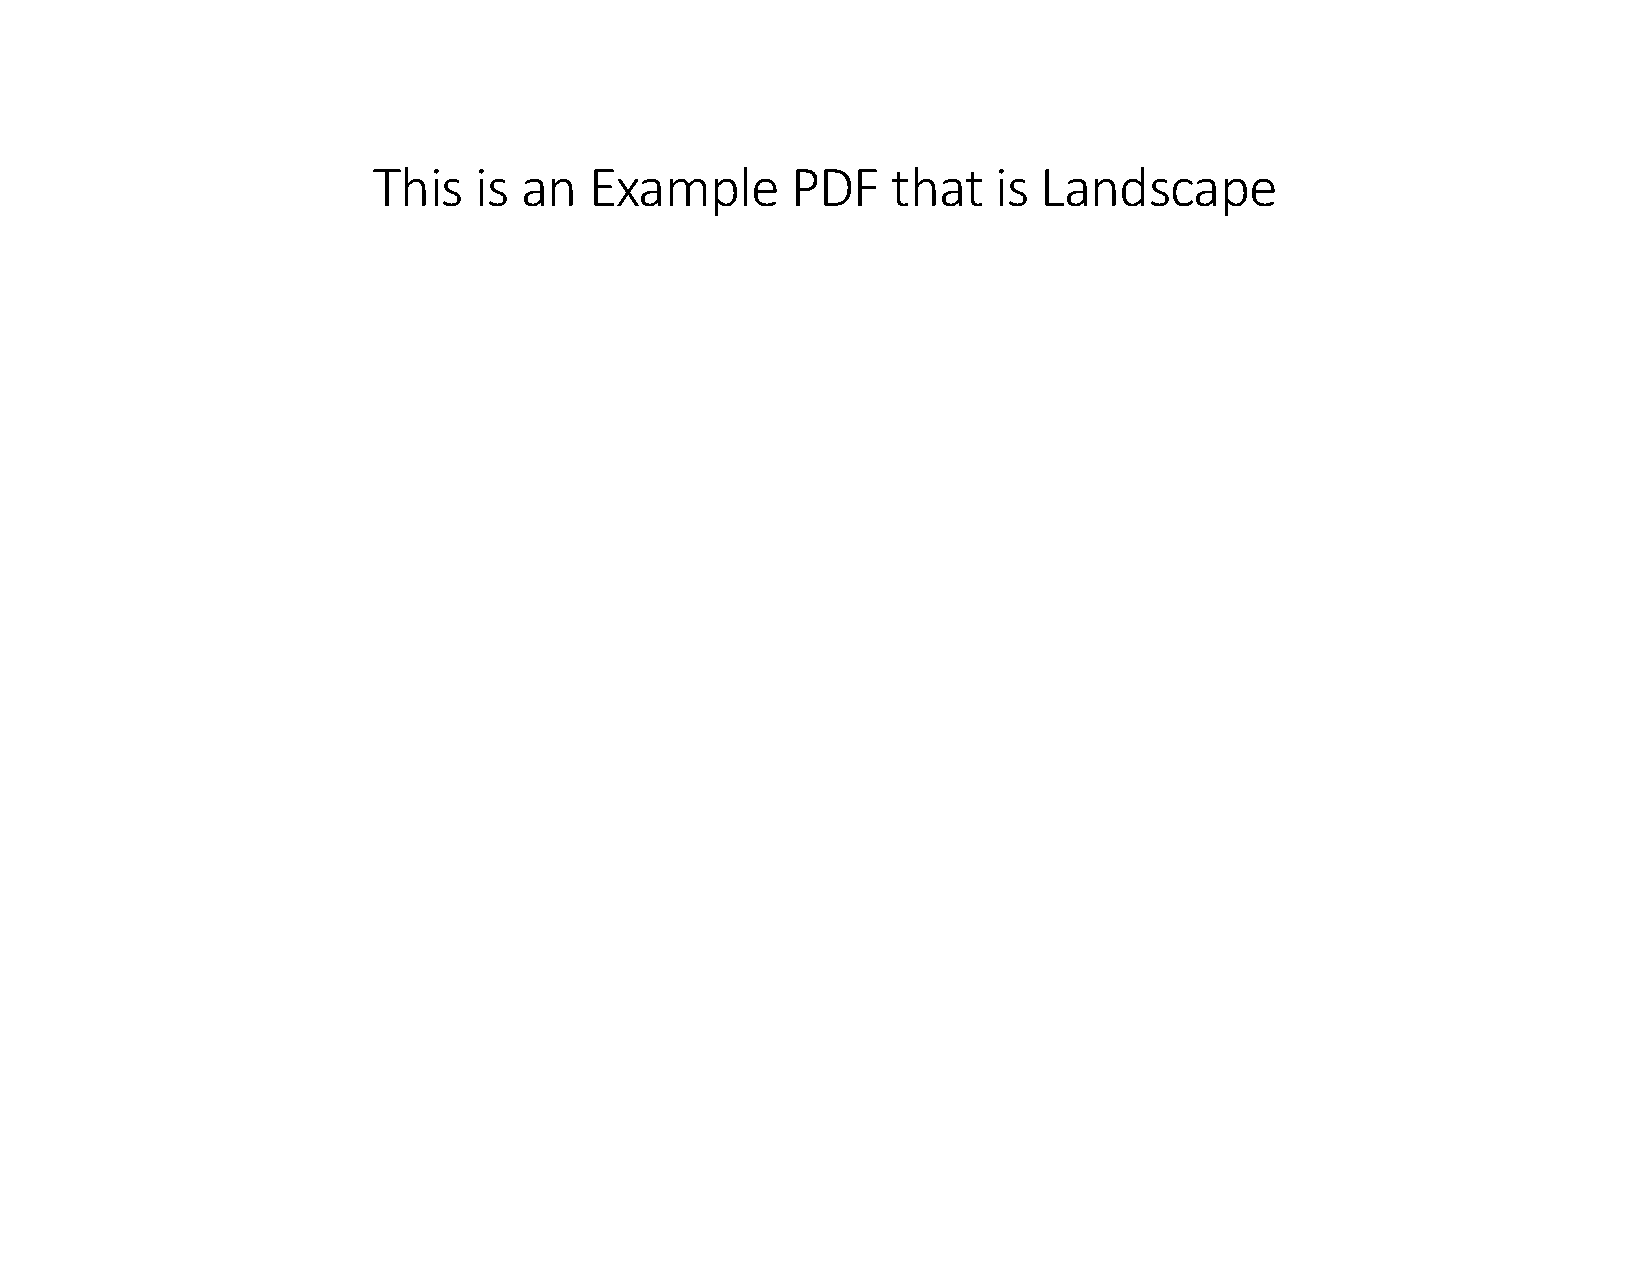
\includepdf[landscape=true,pages=-,pagecommand={},scale=0.85]{./Appendices/landscapePDF}

\end{document}
